\chapter{Implementierung}

Aufbau: Alte Architektur (hier auch Anpassug an Roboter GO für Gamplay (scan, kollision, etc)), Neue
Architektur anhand von a)

(Technische Anforderungen)

Die Architektur des CTGameStudio in der Erstversion musste angepasst werden, um die Anforderungen
des neuen Spielmodus zu erfüllen. Das Hinzufügen eines zweiten Roboters erfordert, mehrere Instanzen
der blockly-Komponente und des Strategie-Interpreters zu erzeugen (etwas generischer formulieren).
Die gleichzeitige Ausführung mehrerer Strategien muss ermöglicht werden. Die Gameloop und
Roboterspielobjekte müssen so angepasst werden, dass die Roboter sinnvoll miteinander interagieren
und sich so verhalten, dass sinnvolles Gameplay möglich ist. Zudem muss das Spiel Dialoge mit
Formularelementen erweitert werden, und das Speichern und Laden von Daten über HTTP-Schnittstellen
des Servers unterstützen. (Statemanagement, + HTML-Komponenten/Render-Strategie)


\section{Alte Architektur}

Das ctGameStudio ist ein Webanwendung. Der Server liefert Seiten an den Browser aus und bietet
Login-Management. Unterstützt wird dies durch das auf Node.JS und MongoDB basiertem
KeystoneJS-Framework \footnote{https://keystonejs.com}. Die Darstellung und das dynamische Verhalten
des Spiels basiert auf browser-seitig ausgeführtem HTML und CSS, und Javascript. Neben
Standard-HTML-Inputs wird Phaser \footnote{https://phaser.io} genutzt, um mittels WebGL
Spielelemente zu rendern.

\begin{figure} \label{architektur-alt} \caption{Architektur des ctGameStudio in der Erstversion.
  Phaser-Spielobjekte sind rot hervorgehoben. Durchgezogene Linien zeigen Eltern-Kind beziehungen,
  wobei die Elternkomponente das Kind erstellt. Gestrichlte Linien zwischen Komponenten zeigen
  Abhängigkeiten, so dass eine Komponente die andere referenziert und internenen Zustand der
  Komponente verändert.} 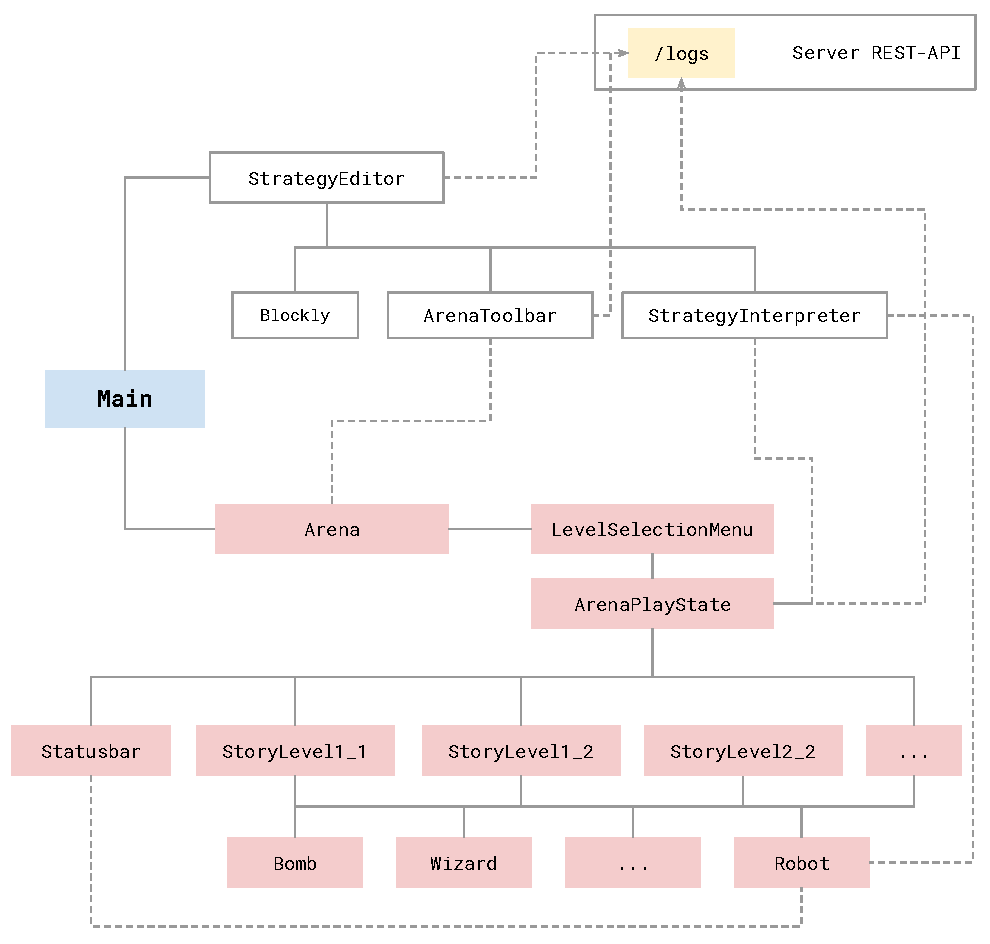
\includegraphics{figures/architektur-alt.pdf} \end{figure}

Komponenten sind als  als Javascript-Funktionen, Objekte oder Klassen definiert. Während eine
Strukturierung dadurch erfolgt, dass Komponenten auf mehrere Dateien aufgeteilt sind, liegen die
Komponenten, Instanzen der Komponenten als auch interne Zustandsvariablen in einem globalen
Namensraum. Dadurch ist direkter Zugriff von eigentlich unabhängigen Komponenten aufeinander möglich
und führt zu einer hohen Kopplung zwischen Komponenten.

\subsection{Main}

Die Hauptfunktion wird nach Laden der Webseite aufgerufen und inialisiert das Phaser-Spiel, welches
das Spielmenü und die Roboter-Umgebung enthält, sowie den Strategieeditor.

\subsection{Strategieeditor}

Der Strategieeditor enthält den Blockly-Oberfläche zur Erstellung eines Programms, den
Strategieinterpreter der für die Ausführung der Strategie zuständig ist, und eine Toolbar mit
Steuerungselemente zur Ausführung der Strategien und Aufruf des Blocklexikons.

\subsection{Blockly}

Die Blockly\footnote{https://developers.google.com/blockly/}-Bibliothek stellt einen Editor zur
blockbasierten Programmierung bereit. Zur Konfiguration des Editors werden die Blöcke
definiert, aus denen der Anwender sein Programm zusammenstellen kann. Die Konfiguration besteht aus
einer mit XML strukturierten Beschreibung der Blöcke, sowie aus Javascript-Funktionen, die
beschreiben, welcher Code aus einem Block generiert werden soll. \todo{Codebeispiel?} Die
Blockly-Developer-Tools\footnote{https://blockly-demo.appspot.com/static/demos/blockfactory/index.html}
können genutzt werden, um die Block-Konfiguration zu generieren und zu verwalten.

Für das ctGameStudio wurden Blöcke definiert, die Aktionen des Roboters entsprechen. Der zu einem
Block zugehörige Code ist ein Funktionsaufruf, der im Aufruf einer Methode des Roboter-Spielobjekts
resultiert (mehr dazu im nächsten Abschnitt).

Die Programme, die mit dem Editor erstellt wurden, können als XML exportiert werden. Analog dazu
kann das Programm in den Editor importiert werden. Zusätzlich kann das Programm in Block-Struktur
andhand der Block-Konfiguration in Javascript-Code umgewandelt werden.

Im ctGameStudio wird der Blockly Editor zur Erstellung von Roboterstrategien genutzt. Bei Laden
eines Storylevels wird die Werkzeugleiste und das bereit stehende Programm dynamisch an die
Anforderungen des Levels angepasst. So sind nur die Blöcke verfügbar, die in dem Level benutzt
werden sollen, und der Editor wird mit einem leeren oder teils vordefiniertem Programm bestückt.

Bei Ausführung der Roboterstrategie wird eine Javascript-Version des Blockprogramms generiert, und
mit dem Strategieinterpreter ausgeführt.

\subsection{Strategieinterpreter}

Der Strategieinterpreter ist dazu da, den aus Blockly generierten Javascript-Code auszuführen, und
so den Roboter auf dem Spielfeld zu steuern. Er basiert auf dem
JS-Interpreter\footnote{https://neil.fraser.name/software/JS-Interpreter/docs.html} von Neil Fraser,
der eine Sandbox-Umgebung zur sicheren Ausführung von Javscript bereit stellt. Das Sandboxing
garantiert, dass der Code isoliert von der Host-Umgebung, also der Javascript-Umgebung in der das
Spiel läuft, ausgeführt werden kann. Der durch den Anwender erstellten Code kann durch seine
Ausführung keine Crashes oder Endlosschleifen verursachen. Der Code bekommt keinen Zugang auf das
DOM. Außerdem wird verhindert, dass der Code übermäßig Speicher belegt.

Neben nativer Javascript-Funktionalität (z.B. Rechenoperationen, Schleifen, und dem Definieren und
Ausführung von Funktionen) gibt der Interpreter die Möglichkeit, Funktionen zu definieren, die aus
der Sandbox heraus aufgerufen werden können. Im ctGameStudio wird dies genutzt, um Befehle zur
Steuerung des Roboters bereit zu stellen. Dazu wird für jede Fähigkeit des Roboters eine Funktion
definiert, die eine zugehörige Methode auf dem Roboter-Spielobjekt ausführt.

Bei Ausführung der Strategie wird der Strategiecode in den Interpreter geladen. Dieser stellt dann
eine Funktion bereit, mit der Code schrittweise ausgeführt werden kann. Eine eigens definierte
Schritt-Funktion ist dafür da, den Code so lange auszuführen, bis jeder Befehl abgearbeitet wurde,
bis der Roboter zerstört wurde, oder bis der Roboter als \enquote{busy} markiert wurde. Letzteres
ist immer dann der Fall, wenn der Roboter einen Befehl ausführt. Die Wiederholung wird durch einen
rekursiven Aufruf der Schritt-Funktion hervorgerufen. Wenn der Interpreter viele Befehle ohne
Unterbrechung abarbeitet, kann dies einen Stack Overflow hervorrufen, was Fehlfunktionen der
Strategieausführung nach sich zieht.

Die Schritt-Funktion wird initial beim Start der Ausführung durch den Nutzer aufgerufen. Daraufhin
wird die Funktion immer nach Abschluss einer Aktion des Roboters oder wenn durch ein Spielereignis
(z.B. Kollision mit dem Rand der Spielwelt) die gerade ausgeführte Aktion des Roboters unterbrochen
wurde.

\todo{Diagramm + Pseudo-Code der Ausführung}


\section{Anpassung der Architektur}

Das CTGameStudio in der Erstversion besteht aus zwei lose definierten Haupt-Komponenten (Abb. 1).
Das Menü und die Arena sind ein Phaser-Spiel, in dem Untermenüs und die Spielfläche (Arena) als
unterschiedliche Phaser-States implementiert sind. Der Strategieeditor, die Strategieausführung und
die Toolbar zum Starten und Stoppen der Strategien sind in einer blockly-Komponente gebündelt. Die
Interaktion zwischen den Komponenten fand über globale Variablen und Funktionen statt, wodurch

Beim Start des CTGameStudios werden beide Komponenten initialisiert. Zu Beginn eines Spiellevels
wird der Editor vom Arena-state zurückgesetzt, so dass er ausschließlich die Blöcke und die leere
oder zum Teil gefüllte Stratgie enthält, mit denen der Lernende die Strategie für das Level
entwickeln soll.

Bei Hinzufügen, Verändern oder Entfernen von Blöcken wird der Javascript-Code zur Steuerung des
Roboters generiert und in den Strategie-Interpreter geladen.


- Refactoring: Modularisierung und Entkopplung um Wartbarkeit zu erhöhen, neue Features einfacher
einbauen zu können - Verstärkte Modularisierung durch Bündeln von Dingen die zusammen gehören -
Strategie-Editor war gebündelt mit Strategie-Interpreter, der die Roboter-Strategie ausführt, der
API des Roboter-Spielobjekts die vom Stratgie-Interpreter, und User Interface-Steuerung - und
verpacken in nativen Javascript, so dass funktionen und Variablen eines Moduls exportiert und von
anderen Modulen importiert werden kann - 


Vorher: Loses html, Spiel-Menü + Arena in Phaser, blockly-Komponente intermingled mit Ausführung des
Codes, (Key-Terms: Main, RoboInterpreter, RoboProgrammer, Menü, Arena, Statusleiste), starke
Kopplung

Einbinden eines zweiten Roboters

Formulare, Turnierplugin, Design -> HTML-Komponenten (Menüs, Statusbar, Toolbar) Phaser nur noch
Arena Modularisierung Entkopplung über Main

Server bekommt neue Rolle, nicht lediglich Bereitstellen von Login und Ausliefern der Seite, sondern
API und Persistenz

\section{Ausführung der Strategien}

- Gameplay erfordert klare, deterministische Koordination zwischen Strategieinterpreter und Gameloop
-> Interpreter nicht parallel zu Gameloop ausführen sondern aus Gameloop aufgerufen

\section{Zustandsmanagement}

Durch neue Dialoge und Interaktionsmöglichkeiten und Kommunikation mit dem Server hat das Spiel an
Komplexität zugenommen. Um trotzdem einfache Wartbarkeit und Erweiterbarkeit des Spiels zu
gewährleisten, wurde ein System zum Management des Programmzustands eingeführt. Als Zustand des
Programms werden die Parameter bezeichnet, die bestimmen, welche Komponenten gerendert werden und
welche Daten diese erhalten.
% Damit wird bestimmt, wie des Spiel zu einem bestimmten Zeitpunkt aussieht, wie es sich verhält,
% und welche Aktionen vom Nutzer entegegen genommen werden können.

...Walkthrough mit Abbildung.... Der initiale Programmzustand bildet also die Daten ab, die die
Komponenten so konfigurieren, dass diese das erste Menü anzeigen.

Änderungen des Zustands werden durch die Abhandlung von \em{Aktionen} herbeigeführt, die auf Aufruf
von Update-Funktionen mappen. Rendering top down, actions up

Immutability, Main-Methode (Besitz/Kontrolle des States) Die main-Funktion enthält die Referenz auf
den Zustand und gibt ihn an.

Vorteile: - Sichtbarkeit von Änderungen führt zu hoher Debugability - Zustandsänderungen durch pure
Funktionen erhöht Testbarkeit und Argumentation über Veränderungen


\begin{lstlisting}{Ausschnitt aus Zustandsmodell} \end{lstlisting}

\subsection{Zustandsmanagement der Phaser-Komponente}

Das Phaser-Framework gibt einen Update-Render-Loop vor, der sich von Funktionsweise des
Update-Render-Loops des in HTML implementierten Teils unterscheidet. Das Framework ruft
kontiniuierlich eine Update-Funktion auf, in der Spielobjekte hinzugefügt und entfernt werden und
Eigenschaften dieser Spielobjekte verändert werden. Das Framework sorgt für das rendering dieser
Objekte.

Key-differences: Objekte sind veränderlich (mutable), Update wird ständig aufgerufen (da sich auch
ständig etwas ändert)

Integration durch ein Event-Interface, welches wiederrum in Actions resultiert welche den
Haupt-Programmzustand verändern. So können beide Welten die Architektur wählen, die am besten zu
ihrem Anwendungszweck passen.

Abbildung State change der zur Anzeige des Spiels führt, Events während des Spiels (onHit),
onFinished.


\subsection{Datenmodell und Client-Server-Kommunikation}

- Strategien, Turnier, Teilnahmen - RESTful API

\section{Anpassung der Gameloop}

- Kollision - Scanvorgang - Geschwindigkeit der Roboter

